\documentclass{article}
\usepackage{mainPoly}

\title{Suites Numériques}
\author{Première Spécialité Mathématiques}
\date{}

\begin{document}
\maketitle
\section{Définition d'une suite}
\begin{tcolorbox}
\begin{definition}
Une \textbf{suite numérique réelle} est une fonction $u$ définie sur $\N$ à valeurs dans $\R$. Pour tout $n \in \N$, on note l'image $u(n)$ sous le format $u_n$, qui se lit \emph{\og $u$ indice $n$ \fg}. Cette image est appellée \textbf{terme de rang $n$ de $u$}.
\end{definition}
\end{tcolorbox}
\begin{example}
De nombreux phénomènes ne présentent pas de continuité, et peuvent être modélisés par des suites.
\begin{itemize}
\item Le chiffre d'affaire d'une entreprise $n$ mois après sa création.
\item Le nombre de façons de ranger $n$ figurines sur une étagère.
\item L'aire de la figure suivante après la $n$-ième étape.
\begin{center}
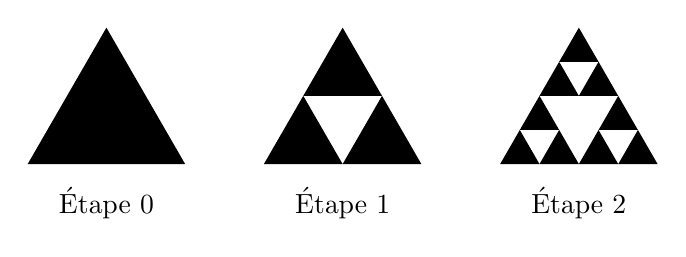
\begin{tikzpicture}
\fill (0,0) -- ++(0:2) -- ++(120:2);

\fill (3,0) -- ++(0:1) -- ++(120:1);
\fill (4,0) -- ++(0:1) -- ++(120:1);
\fill (3,0) ++(60:1) -- ++(0:1) -- ++(120:1);

\fill (6,0) -- ++(0:0.5) -- ++(120:0.5);
\fill (6.5,0) -- ++(0:0.5) -- ++(120:0.5);
\fill (7,0) -- ++(0:0.5) -- ++(120:0.5);
\fill (7.5,0) -- ++(0:0.5) -- ++(120:0.5);
\fill (6,0) ++ (60:0.5) -- ++(0:0.5) -- ++(120:0.5);
\fill (7,0) ++ (60:0.5) -- ++(0:0.5) -- ++(120:0.5);

\fill (6,0) ++ (60:1) -- ++(0:0.5) -- ++(120:0.5);
\fill (6,0) ++ (60:1) ++(0:0.5) -- ++(0:0.5) -- ++(120:0.5);
\fill (6,0) ++ (60:1) ++(60:0.5) -- ++(0:0.5) -- ++(120:0.5);

\draw (1,-0.5) node {Étape $0$};
\draw (4,-0.5) node {Étape $1$};
\draw (7,-0.5) node {Étape $2$};
\end{tikzpicture}
\end{center}
\end{itemize}
\end{example}
\begin{remark}
Une suite peut-être présentée sous la forme d'une séquence de nombres. Dans ce cas, le premier nombre de cette liste correspond au terme d'indice $0$.
\end{remark}
\begin{tcolorbox}
Pour parler d'une suite $u$ en toute généralité, on la note $(u_n)_{n \in \N}$.
\end{tcolorbox}
\begin{remark}
Ainsi, on ne confondra pas les notations $(u_n)_{n \in \N}$ (la suite en toute généralite) et $u_n$ (le $n$\ieme{} terme de la suite).
\end{remark}

\begin{definition}
Si l'on connait $f(n)$ une expression dépendant de $n$ telle que pour tout $n$, $u_n = f(n)$, alors on dit que la suite $(u_n)_{n \in \N}$ est définie de façon \textbf{explicite}.
\end{definition}
\begin{example}
Pour chacune des définitions explicites de $(u_n)_{n \in \N}$ données ci-dessous, donner les 4 premiers termes $u_0; u_1; u_2$ et $u_3$.
\begin{itemize}
\item $u_n = 3n + 1$ pour tout $n \in \N$ : \answersline
\item $u_n = 5 \times 2^n$ pour tout $n \in \N$ : \answersline
\item $u_n = \text{\og Le nombre de lettres dans l'écriture en français de $n$ \fg}$, pour tout $n \in \N$ : \answersline
\end{itemize}
\end{example}
\begin{tcolorbox}
\begin{definition}
Soit $(u_n)_{n \in \N}$ une suite numérique. On dit que $u_n$ est définie \textbf{par récurrence} si $u_0$ est connue, et si pour tout $n \in \N$, le terme $u_{n+1}$ est obtenu en fonction de $u_n$.  
\end{definition}
\end{tcolorbox}
\begin{example}
Pour chacune des définition par récurrence de $(v_n)_{n \in \N}$, calculer les $4$ premiers termes $v_0; v_1; v_2$ et $v_3$.
\begin{itemize}
\item $v_0 = 6$ et $v_{n+1} = v_n + 4$ : \answersline
\item $v_0 = 2$ et $v_{n+1} = 5 \times v_n$ : \answersline 
\end{itemize}
\end{example}
\newpage
\section{Étude de suites}
\subsection{Représentation graphique}
Soit $(u_n)_{n \in \N}$ une suite numérique. Pour représenter $(u_n)_{n \in \N}$ sur un repère orthonormé, on y fait figurer les points de coordonnées $(n;u_n)$.
\begin{center}
\includegraphics[width=\textwidth]{Repr_suite.png}
\end{center}
\subsection{Variation de suites}
\begin{tcolorbox}
\begin{definition}
Soit $(u_n)_{n \in \N}$ une suite numérique.
\begin{itemize}
\item On dit que $(u_n)_{n \in \N}$ est \textbf{croissante} si et seulement si pour tout $n \in \N$, on a $u_n \leq u_{n+1}$. 
\item On dit que $(u_n)_{n \in \N}$ est \textbf{décroissante} si et seulement si pour tout $n \in \N$, on a $u_{n+1} \leq u_n$. 
\end{itemize}
\end{definition}
\end{tcolorbox}
\begin{proposition}
Soit $(u_n)_{n \in \N}$ une suite numérique.
\begin{itemize}
\item La suite $(u_n)_{n \in \N}$ est croissante si et seulement si, pour tout $n \in \N$, $u_{n+1} - u_n \geq 0$. 
\item La suite $(u_n)_{n \in \N}$ est décroissante si et seulement si, pour tout $n \in \N$, $u_{n+1} - u_n \leq 0$. 
\end{itemize}
\end{proposition}
\begin{example}
Étudier les variations des suites suivantes :
\begin{enumquestions}
\item $(u_n)_{n \in \N}$ définie par $u_n = 8 + 4n$ pour tout $n \in \N$.
\item $(v_n)_{n \in \N}$ définie par $v_0 = 64$ et $v_{n+1} = \dfrac{v_n}{2}$ pour tout $n \in \N$.
\item $(w_n)_{n \in \N}$ définie par $w_n = \dfrac{n}{n+1}$ pour tout $n \in \N$.
\item $(z_n)_{n \in \N}$ définie par $z_n = (-1)^n$ pour tout $n \in \N$.
\end{enumquestions}
\emptybox{6cm}
\end{example}
\newpage
\section{Suites arithmétiques}
\begin{tcolorbox}
\begin{definition}
Soit $(u_n)_{n \in \N}$ une suite numérique. On dit que la suite est \textbf{arithmétique} si et seulement il existe $r \in \R$ tel que
\begin{equation*}
u_{n+1} = u_n + r
\end{equation*}
Dans ce cas, on dit que $(u_n)_{n \in \N}$ est la suite arithmétique de \textbf{premier terme} $u_0$ et de \textbf{raison} $r$.
\end{definition}
\end{tcolorbox}
\begin{remark}
Le calcul des termes d'une suite arithmétique de raison $r \in \R$ peut être schématisé comme suit :
\begin{center}
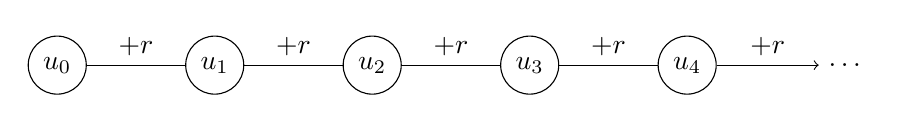
\begin{tikzpicture}
\node[draw,circle] (0) at (0,0) {$u_0$};
\node[draw,circle] (1) at (2,0) {$u_1$};
\node[draw,circle] (2) at (4,0) {$u_2$};
\node[draw,circle] (3) at (6,0) {$u_3$};
\node[draw,circle] (4) at (8,0) {$u_4$};
\node (5) at (10,0) {$\dots$};
\draw[->] 
    (0) -- node[midway,above] {$+r$} 
    (1) -- node[midway,above] {$+r$}
    (2) -- node[midway,above] {$+r$}
    (3) -- node[midway,above] {$+r$}
    (4) -- node[midway,above] {$+r$}
    (5);
\end{tikzpicture}
\end{center}
\end{remark}
\begin{example}
Calculer les termes $u_1$, $u_2$ et $u_3$ pour chaque définition suivante :
\begin{enumquestions}
\item $(u_n)_{n \in \N}$ est la suite arithmétique de premier terme $0$ et de raison $1$ : \answersline
\item $(u_n)_{n \in \N}$ est la suite arithmétique de premier terme $1$ et de raison $2$ : \answersline
\item $(u_n)_{n \in \N}$ est la suite arithmétique de premier terme $10$ et de raison $-\dfrac{1}{2}$ : \answersline
\end{enumquestions}
\end{example}
\begin{proposition}[Variation d'une suite arithmétique]
Soit $(u_n)_{n \in \N}$ une suite arithmétique de raison $r \in \R$.
\begin{itemize}
\item La suite $(u_n)_{n \in \N}$ est croissante si et seulement si $r \geq 0$. 
\item La suite $(u_n)_{n \in \N}$ est décroissante si et seulement si $r \leq 0$. 
\end{itemize}
\end{proposition}
\begin{remark}
Dans le cas particulier où $r = 0$, on dit que la suite $(u_n)_{n \in \N}$ est \textbf{constante}.
\end{remark}
\begin{proposition}[Formule explicite d'une suite arithmétique]
Soit $(u_n)_{n \in \N}$ une suite arithmétique de raison $r \in \R$. Alors, pour tout $n \in \N$, on observe
\begin{equation*}
u_n = u_0 + n \times r
\end{equation*}
\end{proposition}
\begin{remark}
On peut résumer cette formule à l'aide du schéma suivant :
\begin{center}
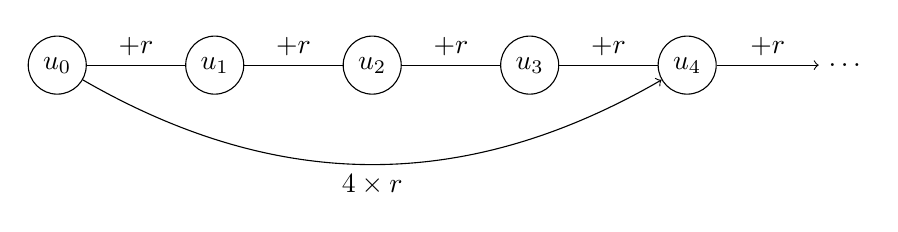
\begin{tikzpicture}
\node[draw,circle] (0) at (0,0) {$u_0$};
\node[draw,circle] (1) at (2,0) {$u_1$};
\node[draw,circle] (2) at (4,0) {$u_2$};
\node[draw,circle] (3) at (6,0) {$u_3$};
\node[draw,circle] (4) at (8,0) {$u_4$};
\node (5) at (10,0) {$\dots$};
\draw[->] 
    (0) -- node[midway,above] {$+r$} 
    (1) -- node[midway,above] {$+r$}
    (2) -- node[midway,above] {$+r$}
    (3) -- node[midway,above] {$+r$}
    (4) -- node[midway,above] {$+r$}
    (5);
\draw[->] (0) to[bend right] node[midway,below] {$4 \times r$} (4);
\end{tikzpicture}
\end{center}
\end{remark}
\begin{example}
Pour chacune des définitions suivantes de $(u_n)_{n \in \N}$, calculer $u_{10}$ :
\begin{enumquestions}
\item $(u_n)_{n \in \N}$ est la suite arithmétique de premier terme $6$ et de raison $5$ : \answersline
\item $(u_n)_{n \in \N}$ est la suite arithmétique de premier terme $0$ et de raison $-2$ : \answersline
\item $(u_n)_{n \in \N}$ est la suite arithmétique de premier terme $1$ et de raison $\dfrac{1}{5}$ : \answersline
\end{enumquestions}
\end{example}
\begin{tcolorbox}
\begin{proposition}
Si $(u_n)_{n \in \N}$ est une suite arithmétique, alors les points de sa représentation graphique sont alignés sur la droite d'équation $y = rx + u_0$ :
\begin{center}
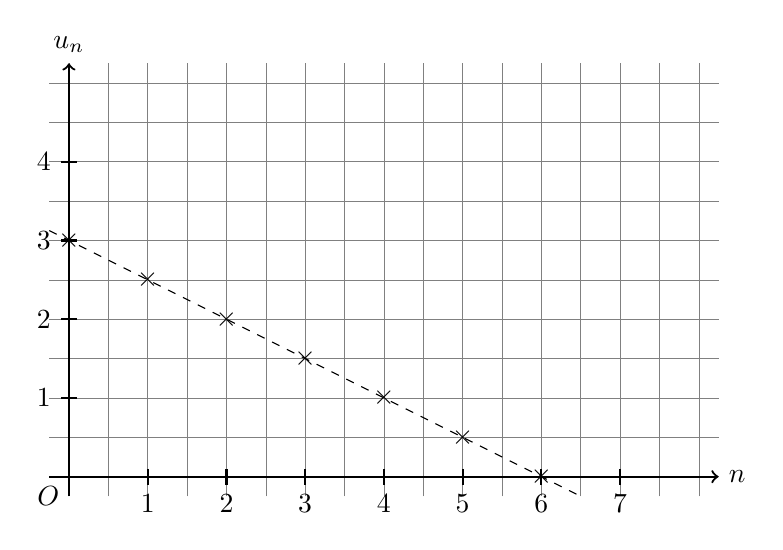
\begin{tikzpicture}
\draw[help lines] (-0.25,-0.25) grid[step=0.5] (8.25,5.25);
\draw[thick,->] (0,-0.25) -- (0,5.25) node[above] {$u_n$};
\draw[thick,->] (-0.25,0) -- (8.25,0) node[right] {$n$};
\foreach \x in {1,...,7}
{\draw[thick] (\x,0.1) -- (\x,-0.1) node[below] {$\x$};}
\foreach \x in {1,...,4}
{\draw[thick] (0.1,\x) -- (-0.1,\x) node[left] {$\x$};}
\draw (0,0) node[below left] {$O$};

\draw (0,3) node {$\times$};
\draw (1,2.5) node {$\times$};
\draw (2,2) node {$\times$};
\draw (3,1.5) node {$\times$};
\draw (4,1) node {$\times$};
\draw (5,0.5) node {$\times$};
\draw (6,0) node {$\times$};
\draw[dashed] (-0.25,3.125) -- (6.5,-0.25);
\end{tikzpicture}
\end{center}
On dit que les suites arithmétiques permettent de modéliser des \textbf{évolutions linéaires}. 
\end{proposition}
\end{tcolorbox}

\newpage
\section{Suites géométriques}
\begin{tcolorbox}
\begin{definition}
Soit $(u_n)_{n \in \N}$ une suite numérique. On dit que la suite est \textbf{géométrique} si et seulement il existe $q \in \R$ tel que
\begin{equation*}
u_{n+1} = u_n \times q
\end{equation*}
Dans ce cas, on dit que $(u_n)_{n \in \N}$ est la suite géométrique de \textbf{premier terme} $u_0$ et de \textbf{raison} $q$.
\end{definition}
\end{tcolorbox}
\begin{remark}
Le calcul des termes d'une suite géométrique de raison $q \in \R$ peut être schématisé comme suit :
\begin{center}
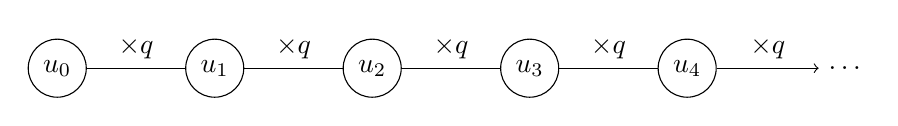
\begin{tikzpicture}
\node[draw,circle] (0) at (0,0) {$u_0$};
\node[draw,circle] (1) at (2,0) {$u_1$};
\node[draw,circle] (2) at (4,0) {$u_2$};
\node[draw,circle] (3) at (6,0) {$u_3$};
\node[draw,circle] (4) at (8,0) {$u_4$};
\node (5) at (10,0) {$\dots$};
\draw[->] 
    (0) -- node[midway,above] {$\times q$} 
    (1) -- node[midway,above] {$\times q$}
    (2) -- node[midway,above] {$\times q$}
    (3) -- node[midway,above] {$\times q$}
    (4) -- node[midway,above] {$\times q$}
    (5);
\end{tikzpicture}
\end{center}
\end{remark}
\begin{example}
Calculer les termes $u_1$, $u_2$ et $u_3$ pour chaque définition suivante :
\begin{enumquestions}
\item $(u_n)_{n \in \N}$ est la suite géométrique de premier terme $1$ et de raison $2$ : \answersline
\item $(u_n)_{n \in \N}$ est la suite géométrique de premier terme $64$ et de raison $\dfrac{1}{2}$ : \answersline
\item $(u_n)_{n \in \N}$ est la suite géométrique de premier terme $1000$ et de raison $-0,1$ : \answersline
\end{enumquestions}
\end{example}
\begin{proposition}[Variation d'une suite géométrique]
Soit $(u_n)_{n \in \N}$ une suite géométrique de raison $q \in \R$. \textbf{On suppose que son premier terme $u_0$ est non nul}.
\begin{itemize}
\item Si $q > 1$ :
\begin{itemize}
\item Si $u_0 > 0$, alors $(u_n)_{n \in \N}$ est strictement croissante.
\item Si $u_0 < 0$, alors $(u_n)_{n \in \N}$ est strictement décroissante.
\end{itemize}
\item Si $0 < q < 1$ : 
\begin{itemize}
\item Si $u_0 > 0$, alors $(u_n)_{n \in \N}$ est strictement décroissante.
\item Si $u_0 < 0$, alors $(u_n)_{n \in \N}$ est strictement croissante. 
\end{itemize}
\item Si $q = 0$ ou $q = 1$, alors $(u_n)_{n \in \N}$ est constante à partir du terme $u_1$.
\item Si $q < 0$, alors la suite n'est pas \textbf{monotone} (elle n'est ni croissante, ni décroissante).
\end{itemize}
\end{proposition}
\begin{proposition}[Formule explicite d'une suite géométrique]
Soit $(u_n)_{n \in \N}$ une suite géométrique de raison $q \in \R$. Alors, pour tout $n \in \N$, on observe
\begin{equation*}
u_n = u_0 \times q^n
\end{equation*}
\end{proposition}
\begin{remark}
On peut résumer cette formule à l'aide du schéma suivant :
\begin{center}
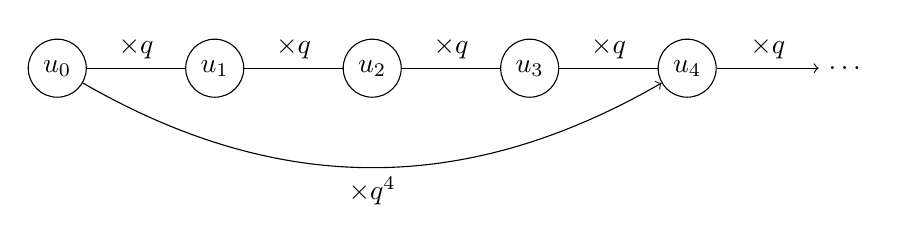
\begin{tikzpicture}
\node[draw,circle] (0) at (0,0) {$u_0$};
\node[draw,circle] (1) at (2,0) {$u_1$};
\node[draw,circle] (2) at (4,0) {$u_2$};
\node[draw,circle] (3) at (6,0) {$u_3$};
\node[draw,circle] (4) at (8,0) {$u_4$};
\node (5) at (10,0) {$\dots$};
\draw[->] 
    (0) -- node[midway,above] {$\times q$} 
    (1) -- node[midway,above] {$\times q$}
    (2) -- node[midway,above] {$\times q$}
    (3) -- node[midway,above] {$\times q$}
    (4) -- node[midway,above] {$\times q$}
    (5);
\draw[->] (0) to[bend right] node[midway,below] {$\times q^4$} (4);
\end{tikzpicture}
\end{center}
\end{remark}
\begin{example}
Pour chacune des définitions suivantes de $(u_n)_{n \in \N}$, calculer $u_{10}$ :
\begin{enumquestions}
\item $(u_n)_{n \in \N}$ est la suite géométrique de premier terme $1$ et de raison $-2$ : \answersline
\item $(u_n)_{n \in \N}$ est la suite géométrique de premier terme $5^{10} = \num{9765625}$ et de raison $\dfrac{1}{5}$ : \answersline
\end{enumquestions}
\end{example}
\begin{tcolorbox}
\begin{definition}
Les suites géométriques permettent de modéliser des évolutions dites \textbf{exponentielles}.         
\end{definition}
\end{tcolorbox}
\newpage
\section{Calcul de sommes}
\subsection{Sommes arithmétiques}
\begin{tcolorbox}
\begin{proposition}
Soit $n$ un nombre entier naturel. Alors,
\begin{equation*}
1 + 2 + 3 + \dots + n = \dfrac{n(n+1)}{2}
\end{equation*}
\end{proposition}
\end{tcolorbox}
\begin{proof}
\hfill

\vspace{0.2cm}
\emptybox{5cm}
\end{proof}
\begin{proposition}
Soit $(u_n)_{n \in \N}$ une suite arithmétique de raison $r$, et $N$ un entier naturel. Alors,
\begin{equation*}
u_0 + u_1 + u_2 + \dots + u_N = (N+1)u_0 + \dfrac{N(N+1)r}{2}
\end{equation*}
\end{proposition}
\begin{proof}
\hfill

\vspace{0.2cm}
\emptybox{5cm}
\end{proof}
\begin{example}
Soit $(u_n)_{n \in N}$ une suite arithmétique de premier terme $u_0 = 2$ et de raison $r = 3$. Calculer $u_0 + u_1 + u_2 + \dots + u_{15}$ (somme des 16 premiers termes).

\vspace*{0.2cm}
\emptybox{3cm}
\end{example}

\newpage
\subsection{Sommes géométriques}
\begin{tcolorbox}
\begin{proposition}
Soit $n$ un nombre entier naturel, et $q \neq 1$ un réel. Alors,
\begin{equation*}
1 + q^1 + q^2 + \dots + q^n = \dfrac{1 - q^{n+1}}{1 - q} = \dfrac{q^{n+1} - 1}{q - 1}
\end{equation*}
\end{proposition}
\end{tcolorbox}
\begin{proof}
\hfill

\vspace{0.2cm}
\emptybox{5cm}
\end{proof}
\begin{proposition}
Soit $(u_n)_{n \in \N}$ une suite géométrique de raison $q \neq 1$, et $N$ un entier naturel. Alors,
\begin{equation*}
u_0 + u_1 + u_2 + \dots + u_N = u_0 \dfrac{q^{n+1} - 1}{q - 1}
\end{equation*}
\end{proposition}
\begin{proof}
\hfill

\vspace{0.2cm}
\emptybox{5cm}
\end{proof}
\begin{example}
Soit $(u_n)_{n \in N}$ une suite géométrique de premier terme $u_0 = 3$ et de raison $q = 2$. Calculer $u_0 + u_1 + u_2 + \dots + u_{19}$ (somme des 20 premiers termes).

\vspace*{0.2cm}
\emptybox{3cm}
\end{example}
\newpage
\section{Notion de limite}
\subsection{Convergence de suites}
\begin{tcolorbox}
\begin{definition}[Limite finie d'une suite]
Soit $(u_n)_{n \in \N}$ une suite numérique, et $l$ un nombre réel. On dit que \textbf{la suite $(u_n)_{n \in \N}$ admet $l$ comme limite} quand les nombres $u_n$ sont aussi proches de $l$ que l'on veut à mesure que les indices $n$ sont grands. On le note
\begin{equation*}
\lim_{n \to +\infty} u_n = l 
\end{equation*}
\end{definition}
\end{tcolorbox}
\begin{remark}
\hfill
\begin{itemize}
\item Quand une suite admet une limite finie, on dit que la suite \textbf{converge}.
\item Quand une suite ne converge pas, on dit qu'elle \textbf{diverge}.
\end{itemize}
\end{remark}
\begin{example}
On représente une suite $(u_n)_{n \in \N}$ par les points de coordonnées $(n,u_n)$. 

\begin{center}
\begin{tikzpicture}
\repereclassique{-0.25}{-3.25}{10.25}{3.25}{0.5};
\foreach \x in {0,0.5,...,10.0}
{
    \draw (\x,{2*(-1)^(2*\x)/(\x^2+1) + 1}) node {$\bullet$};
}
\draw[dashed] (-0.25,1) -- (10.25,1) node[right] {$y=2$};
\end{tikzpicture}
\end{center}
\begin{tcolorbox}
La suite $(u_n)$ semble converger vers le réel $2$ : plus $n$ est grand (pour des abscisses de plus en plus grandes), et plus $u_n$ est proche de $2$ (les ordonnées des points sont de plus en plus proche de $2$).
\end{tcolorbox}
\begin{center}
\begin{tikzpicture}
\repereclassique{-0.25}{-3.25}{10.25}{3.25}{0.5};
\foreach \x in {0,0.5,...,10.0}
{
    \draw (\x,{2.5*sin(\x r)}) node {$\bullet$};
}
\end{tikzpicture}
\end{center}
\begin{tcolorbox}
Ici, la suite représentée ne semble pas admettre de limite finie $l$. En effet, les ordonnées des points de coordonnées $(n,u_n)$ ne semblent pas se rapprocher d'une valeur en particulier, à la mesure que $n$ augmente.
\end{tcolorbox}
\end{example}
\newpage
\subsection{Divergence vers l'infini}
\begin{tcolorbox}
\begin{definition}
Soit $(u_n)_{n \in \N}$ une suite numérique. On dit que \textbf{la suite $(u_n)$ admet $+\infty$ comme limite} quand les valeurs de $u_n$ sont de plus en plus grandes à la mesure où $n$ augmente. On le note
\begin{equation*}
\lim_{n \to +\infty} u_n = +\infty 
\end{equation*}
\end{definition}    
\end{tcolorbox}
\begin{tcolorbox}
\begin{definition}
Soit $(u_n)_{n \in \N}$ une suite numérique. On dit que \textbf{la suite $(u_n)$ admet $-\infty$ comme limite} quand les valeurs de $u_n$ sont de plus en plus petites à la mesure où $n$ augmente. On le note
\begin{equation*}
\lim_{n \to +\infty} u_n = -\infty 
\end{equation*}
\end{definition}    
\end{tcolorbox}
\begin{remark}
Une suite admettant $+\infty$ ou $-\infty$ comme limite est dite \textbf{divergente}. Une suite diverge donc dans deux cas :
\begin{itemize}
\item si elle n'admet pas de limite finie;
\item ou si elle admet $+\infty$ ou $-\infty$ comme limite.
\end{itemize}
\end{remark}
\begin{example}
Les deux suites $(u_n)$ et $(v_n)$ représentées ci-après admettent $-\infty$ et $+\infty$ comme limite.
\begin{center}
\begin{tikzpicture}
\repereclassique{-0.25}{-3.25}{10.25}{3.25}{0.5};
\foreach \x in {0,0.5,...,10.0}
{
    \draw (\x,{6*exp(\x - 10) - 3}) node {$\bullet$};
}
\end{tikzpicture}
\end{center}
\begin{center}
\begin{tikzpicture}
\repereclassique{-0.25}{-3.25}{10.25}{3.25}{0.5};
\foreach \x in {0,0.5,...,10.0}
{
    \draw (\x,-0.5*\x+2) node {$\bullet$};
}
\end{tikzpicture}
\end{center}
\end{example}
\end{document}